\chapter{The Model}
\label{chap:The Model}

\section{Theory}

We are interested in connecting the interaction rate of photons with energy E to the pair-production cross section $\sigma_{pair}(s)$ and the spectral density of background photons $n_{\gamma}(\varepsilon)$. The interaction rate of photons with energy E is given by the following equation:

\begin{equation}
    R_{\gamma}(E) = \frac{1}{2}\int_{0}^{\infty}d\varepsilon \,n_{\gamma}(\varepsilon)\int_{-1}^{1}d\mu\,(1-\mu)\,\sigma_{pair}(s)\,\Theta(s-s_{min})
    \label{eq:interaction_rate_first_one}
\end{equation}

Where $s_{min}$ is the threshold energy for pair production, and $\Theta(s-s_{min})$ is the Heaviside step function. It is there to ensure we only integrate over possible energies. The pair-production cross-section $\sigma_{pair}(s)$ is well-known, and is given by the following equation:

\begin{equation}
    \sigma_{\rm pair}(s)=\frac{3}{4}\,\sigma_{{\rm Th}}\, \frac{m_e^2}{s}
     \left[(3-\beta^{4})\ln\frac{1+\beta}{1-\beta}-2\beta(2-\beta^{2})\right]\!,
    \label{eq:sigma-pair}
\end{equation}

Where $\sigma_{\rm Th}$ is the Thomson cross-section, $m_e$ is the electron mass, $\beta = \sqrt{1-4\,m_e^2/s}$, and $s = 2E\varepsilon(1-\mu)$.

From equation \ref{eq:interaction_rate_first_one}, it is convenient to rewrite the integrals in terms of the mandelstam variable $s$, and swap the order of integration. Doing this, we get the following equation:

\newpage

\begin{equation*}
    R_{\gamma}(E) = \frac{1}{8E^2}\int_{0}^{\infty}\frac{d\varepsilon}{\varepsilon^2}\,n_{\gamma}(\varepsilon)\int_{s_{min}}^{4E\varepsilon}ds\,s\,\sigma_{pair}(s) =
    \label{eq:interaction_rate_second_one}
\end{equation*}

\begin{equation}
    = R_{\gamma}(E) = \frac{1}{8E^2}\int_{4m_ec^2}^{4E\varepsilon_{max}}ds\,s\,\sigma_{pair}(s)\int_{\frac{s}{4E}}^{\varepsilon_{max}}\frac{d\varepsilon}{\varepsilon^2}\,n_{\gamma}(\varepsilon)
    \label{eq:interaction_rate_third_one}
\end{equation}

Notice that for a given s, we have $s \leq 4E\varepsilon$, which implies that $\varepsilon \geq \frac{s}{4E}$. This is the reason for the lower limit of the $\varepsilon$-integral. The upper limit of the $\varepsilon$-integral is $\varepsilon_{max}$, which is an arbitrary maximum energy which we expect to find of the background photons.

To find the interaction rate of photons with energy E, we need to know the spectral density of background photons $n_{\gamma}(\varepsilon)$. We will assume that the spectral density of background photons is given by piecewise power-law distributions, given by the following equations:

\begin{equation}
    n_{\gamma}(\varepsilon) = \left\{
    \begin{array}{ll}
        n_0\left(\frac{\varepsilon}{\varepsilon_0}\right)^{-\alpha_1} & \text{for } \varepsilon_{min} \leq \varepsilon \leq \varepsilon_{br} \\
        n_0\left(\frac{\varepsilon_{br}}{\varepsilon_0}\right)^{-\alpha_1}\left(\frac{\varepsilon}{\varepsilon_{br}}\right)^{-\alpha_2} & \text{for } \varepsilon_{br} \leq \varepsilon \leq \varepsilon_{max}
    \end{array}
    \right.
    \label{eq:spectral_density}
\end{equation}
% \chapter{Theory}
% \label{chap:Theory}

% The theory section is not as common to include as the other sections included in this document. Some work is theory-heavy, and it can be beneficial to split the theory part from the background and methodology parts of the document. In this document, we will rather use this section to show some important \LaTeX commands that you are likely to use.

% When you write in \LaTeX, try to just follow the given style. You might not like the exact way of the given style in your document, but if you try to change it with small commands everywhere, you will probably end up with a document that looks worse, and you will spend a lot of time writing \LaTeX code in your document.

% \section{Equations}

% A simple equation or variable can be written within sentences using the dollar sign on each side, for example, writing \verb=$a$= will show up as $a$. The usual way of including an equation on a separate line is either by using double dollar signs, such as this:
% $$E = mc^2$$
% or using the \texttt{equation} environment:
% \begin{equation}
%     E=mc^2
%     \label{eq:Einstein}
% \end{equation}
% \sloppy Note that the \texttt{equation} environment will enumerate the equation, and allow you to add a label that you can refer to later. When labeling the equations, you can refer to them using \verb=\eqref{<label>}=, which will give you an equation reference like Eq.~\eqref{eq:Einstein}.

% The text below shows an example of how to align equations on the equal sign, with only one reference for both. This may be useful for when they are linked and are actually only one equation but splitting them up makes it more readable.
% \begin{equation}
% \begin{aligned}
%         a &= \sin^{2}(\Delta\phi/2) + a \sin^{2}(\Delta\phi/2) \\
%          &= (1+a) \sin^{2}(\Delta\phi/2)
% \end{aligned}
% \label{eq:splitTwoLines}
% \end{equation}
% The whole equation can be referenced as a single equation, Eq.~\eqref{eq:splitTwoLines}. One may also align sub-equations such that they are numbered the same but have a letter differentiating them as shown below\footnote{A footnote explaining something.}. This can be used when they are linked, but you will need to reference both individual parts.

% \begin{subequations}
% \begin{align}
%     \sigma &= \sqrt{\frac{1}{N} \sum_{i=1}^N (x_i - \mu)^2}
%     \label{eq:sd}\\ 
%     \mu &= \frac{1}{N} \sum_{i=1}^N x_i \label{eq:mean}
% \end{align}
% \label{eqn:subeqn}
% \end{subequations}\\
% These equations can be referenced by their specific sub-equation as Eq.~\eqref{eq:sd}, or by the whole group as Eqs.~\eqref{eqn:subeqn}.


% \section{Including figures}

% Figure \ref{fig:qualityDiff} is an example of how to include figures in your \LaTeX document. This is also an example of the difference between a vector-based image format (pdf) and a voxel-based format (png). When possible, always try to use a vector-based image format, as that gives infinite resolution.

% These two figures were created using this simple Python code:

% \lstinputlisting[firstline=1, lastline=17,language=Python]{Figures/createPlot.py}

% So when you create figures using Python, try to save them as pdf, as use the tight boundaries to save some space around the figures.

% \begin{figure}[H]
%   \centering
%   \subfloat[Sinus figure using pdf.]{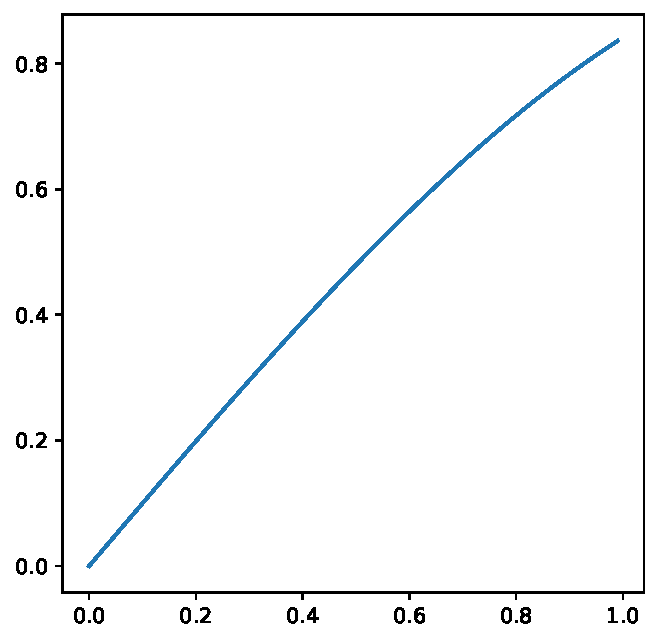
\includegraphics[width=0.45\textwidth]{Figures/sin.pdf}\label{fig:sinpdf}}
%   \quad
%   \subfloat[Sinus figures using png.]{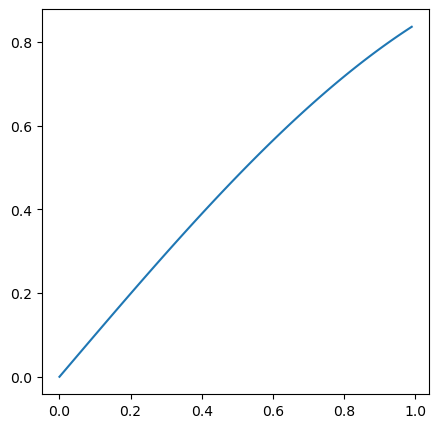
\includegraphics[width=0.45\textwidth]{Figures/sin.png}\label{fig:sinpng}}
%   \caption{Figure (a) shows a pdf figure, while figure (b) shows a png figure. If you zoom in, you will start noticing the difference in quality.}
% \label{fig:qualityDiff}
% \end{figure}

% With Python you could change the size of your figures. This is helpful for getting the right size of text within figures. In Figure \ref{fig:SizeDiff} we compare two different sizes.

% \begin{figure}[H]
%   \centering
%   \subfloat[Sinus figure using size (8,8).]{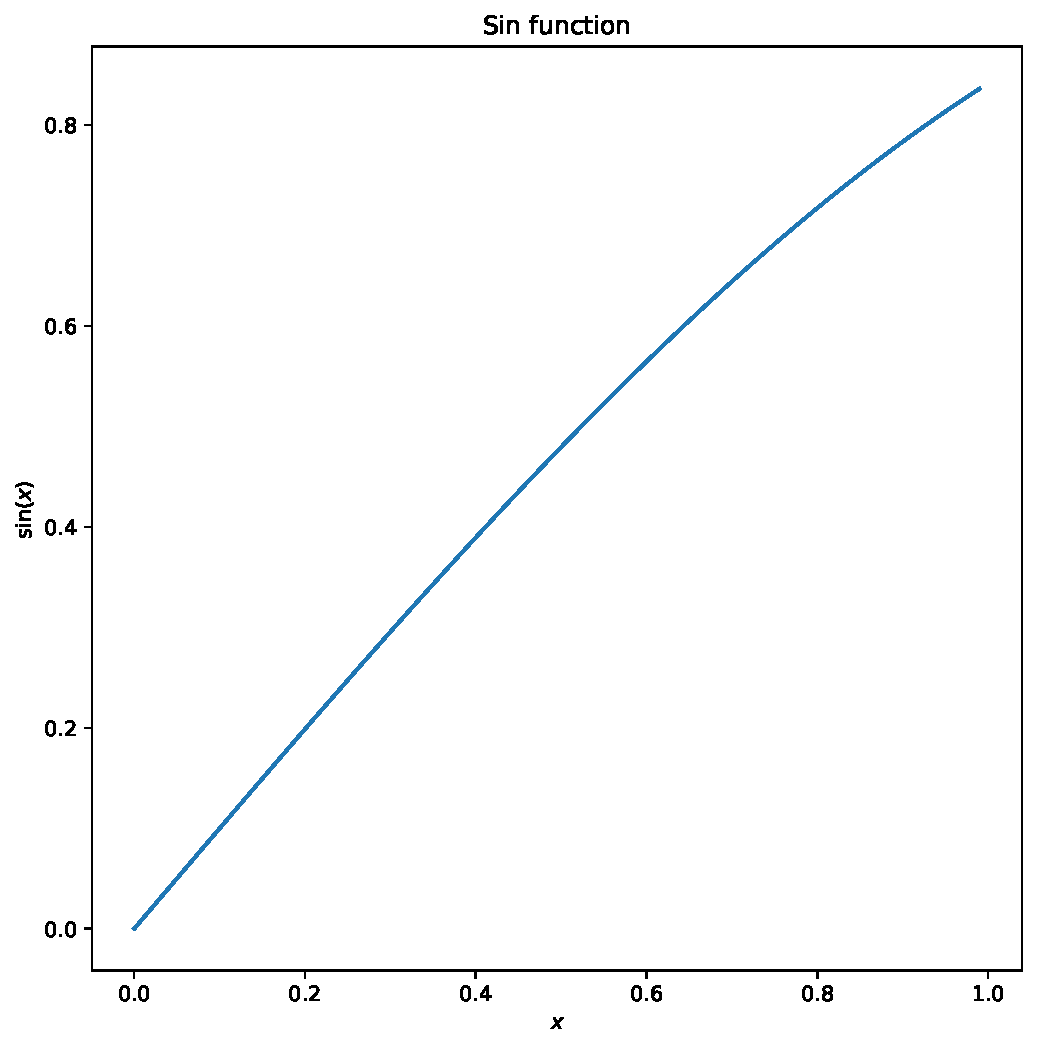
\includegraphics[width=0.45\textwidth]{Figures/sinBig.pdf}\label{fig:sinBig}}
%   \quad
%   \subfloat[Sinus figures using size (4,4).]{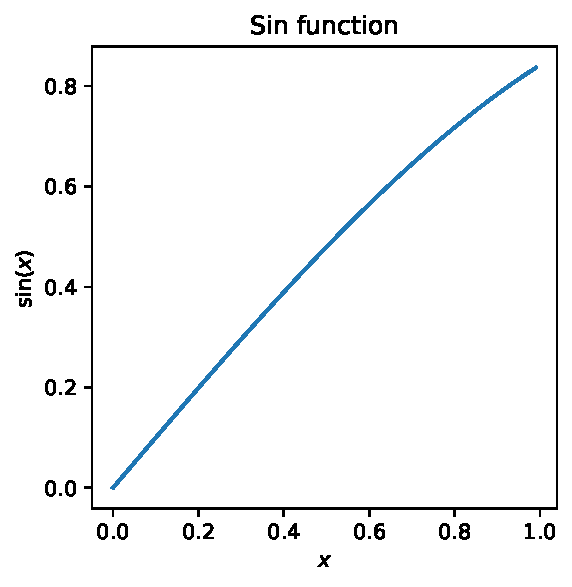
\includegraphics[width=0.45\textwidth]{Figures/sinSmall.pdf}\label{fig:sinSmall}}
%   \caption{This is a comparison between two different figure sizes.}
% \label{fig:SizeDiff}
% \end{figure}


% \section{Chemical notations and units}

% This document has included a package for chemical symbols, \texttt{mchem}. When you write \verb=\ce{CO2}= you will get the chemical notation as \ce{CO2}.

% For units we use the \texttt{siunitx} package. If you write \verb=\SI{10}{\meter\per\second\squared}= you get \SI{10}{\meter\per\second\squared}. The package can be used within math mode (inside the dollar signs). It automatically changes to a fixed notation for numbers, such as \verb=\SI{1E5}{\meter}= gives \SI{1E5}{\meter}.

% \section{Tables}

% Here are two examples of regular tables with data and a table with split headers.

% \begin{table}[ht!]
% \centering
%     \begin{tabular}{ m{3cm} m{2.5cm} m{2.5cm} m{2.5cm} m{2cm} } 
%     \toprule
%     \toprule
%     \textbf{Statistic} & \textbf{Velocity} & \textbf{Altitude} & \textbf{1/Angle} & \textbf{Temp.} \\
%     \midrule
%     Mean    & 122.68    & 240.98   & 93.75     & 13.95 \\[1.3ex]
%     Std     & 224.51    & 145.88   & 60.39     & 4.44  \\[1.3ex]
%     Q1      & 28.00     & 111.60   & 34.15     & 10.60 \\[1.3ex]
%     Median  & 63.00     & 223.20   & 99.59     & 13.30 \\[1.3ex]
%     Q3      & 137.00    & 359.10   & 151.99    & 16.70 \\[1.3ex]
%     Min     & 0.00      & 1.00     & 0.00      & 3.30  \\[1.3ex]
%     Max     & 14519.00  & 616.70   & 180.00    & 32.10 \\[1.3ex]
%     \bottomrule
%     \bottomrule
%     \end{tabular}
% % the square brackets after \caption gives the table a proper title in the list of tables, instead of just inserting the beginning of the table caption
% \caption[Dynamic feature statistics with outliers]{Table of dynamic feature statistics where outliers are included, for all data points. Velocity is given in \textit{m/h}, the altitude in \textit{mamsl}, the inverse trajectory angle in 1/degrees, and temperature in degrees Celsius.}
% \label{table:stat_fliers}
% \end{table}


% \begin{table}[ht!]
% \centering
%     \begin{tabular}{ m{3cm} m{5cm} m{3cm} } 
%     \toprule
%     \toprule
%     \textbf{Area 1} & \textbf{Start date} & \textbf{End date} \\
%     \midrule
%     2018    & 03.06    & 29.06                       \\[1.3ex]
%     2019    & 03.06    & 03.07 or 31.08\footnotemark \\[1.3ex]
%     2020    & 03.06    & 05.09                       \\[1.3ex]
%     \midrule
%     \textbf{Area 2} & \textbf{Start date (farm 1/2)} & \textbf{End date} \\
%     \midrule
%     2012    & 09.06            & 07.09               \\[1.3ex]
%     2013    & 23.06 / 15.06    & 25.08               \\[1.3ex]
%     2014    & 05.06 / 25.06    & 10.09               \\[1.3ex]
%     2015    & 13.06 / 03.07    & 06.09               \\[1.3ex]
%     2016    & 17.06            & 22.07               \\[1.3ex]
%     \bottomrule
%     \bottomrule
%     \end{tabular}
% \caption[Selected time ranges for all data]{Selected time ranges for the data in all areas and all years.}
% \label{table:time_ranges}
% \end{table}

% There are online tools to create \LaTeX tables. This might be a faster way of creating them than writing all the code yourself.
